\section{Hardware}
\label{Sec:hardware}
\subsection{Módulo sensor}

O módulo sensor vai ser responsável por medir e transmitir as informações necessárias para calcular o consumo de energia do equipamento acoplado.

Os componentes físicos do módulo sensor são:

\begin{itemize}
\item Circuito Verificador de tensão
\item Sensor de Corrente (Non-invasive AC Current Sensor)
\item Arduino Uno - R3
\item XBee Shield
\item XBee 2mW PCB Antenna - Series 2
\end{itemize}
%
\subsection{Coordenador}

O módulo coordenador vai ser responsável por fazer requisições para os módulos sensores, tratar os dados de consumo e enviar ao aplicativo na nuvem.

Os componentes do coordenador são:

\begin{itemize}
\item Kit Raspberry Pi2 + Fonte + Microsd 8gb + Wifi Usb
\item XBee Explorer Dongle
\item XBee 2mW PCB Antenna - Series 2
\end{itemize}
%
\subsection{Circuitos}
\subsubsection{Verificador de Tensão}

No circuito de cada módulo de sensor, são feitas detecções da tensão (127V ou 220V) para cálculos de potência.  O objetivo do circuito da figura \ref{fig:voltage-circuit} é indicar se a tensão na tomada é 220V ou 127V. A saída do circuito é usada como um valor analógico, que dependendo da tensão de entrada resultará em faixas diferentes para as diferentes tensões.

\begin{figure}[H]
\centering
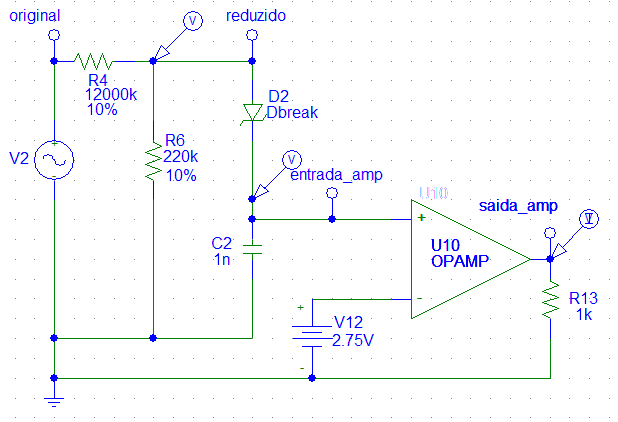
\includegraphics[width=9cm,keepaspectratio]{figuras/voltage-circuit.png}
\caption{\label{fig:voltage-circuit} Circuito verificador de tensão}
\end{figure}

\subsubsection{Medidor de Corrente}

Ainda no módulo sensor, é necessário obter as medidas do valor eficaz da corrente. O sensor não-invasivo produz uma tensão alternada na saída, e antes da coleta de dados pelo arduino é preciso obter um valor significativo, que não ultrapasse 2.5V. Para isso foi utilizado o circuito da figura \ref{fig:sensor-circuit}.

\begin{figure}[H]
\centering
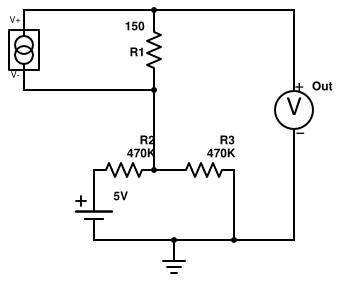
\includegraphics[width=9cm,keepaspectratio]{figuras/current-circuit.jpg}
\caption{\label{fig:sensor-circuit} Circuito medidor de corrente}
\end{figure}
%
\subsection{Peças}
\subsubsection{Sensor de Corrente Não-invasivo AC}

Esse sensor de corrente (figura \ref{fig:sensor}) consegue medir a corrente que passa por um fio de modo não-invasivo. O sensor é um transformador de corrente respondendo ao campo magnético formado em volta do fio condutor. Este, em particular, suporta até 30A de entrada, e necessita de um resistor de saída para obter a medida desejada em tensão \cite{non_invasive_sensor}.

\begin{figure}[H]
\begin{center}
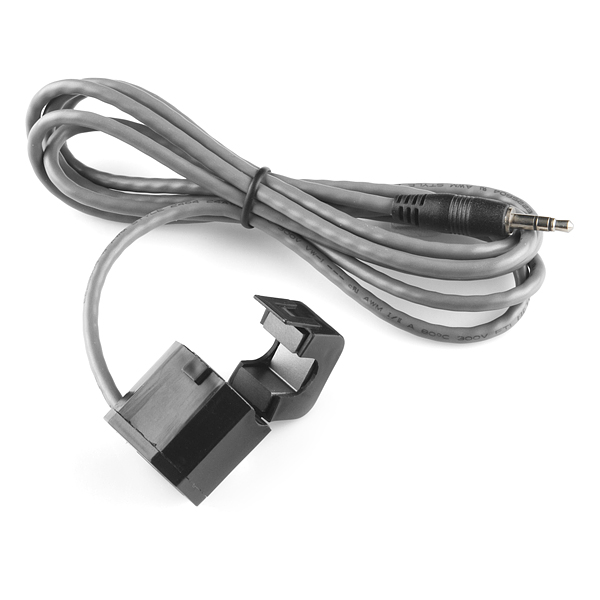
\includegraphics[width=5cm,height=5cm,keepaspectratio]{figuras/sensor.jpg}
\caption{\label{fig:sensor} Non-invasive AC current sensor}
\end{center}
\end{figure}

\begin{itemize}
\item{Corrente suportada: 30A}
\item{Temperatura de operação: -40$^{\circ}$C até 65 $^{\circ}$C}
\item{Precisão de 2\%}
\end{itemize}
%
\subsubsection{Raspberry Pi 2 modelo B}

A Raspberry Pi 2 Modelo B (figura \ref{fig:raspberry pi}) é o computador utilizado no sistema para receber os dados enviados pelos módulos sensores, tratá-los e enviar para o aplicativo. Foi escolhido o Raspberry Pi 2 - Model B por ser mais veloz, por possuir mais entradas USB e ser de alta disponibilidade no mercado, por um preço razoável. O kit inclui a fonte, um cartão microSD de 8GB e um adaptador Wifi USB. Das características do raspberry, pode-se citar \cite{raspberry_datasheet}:

\begin{figure}[H]
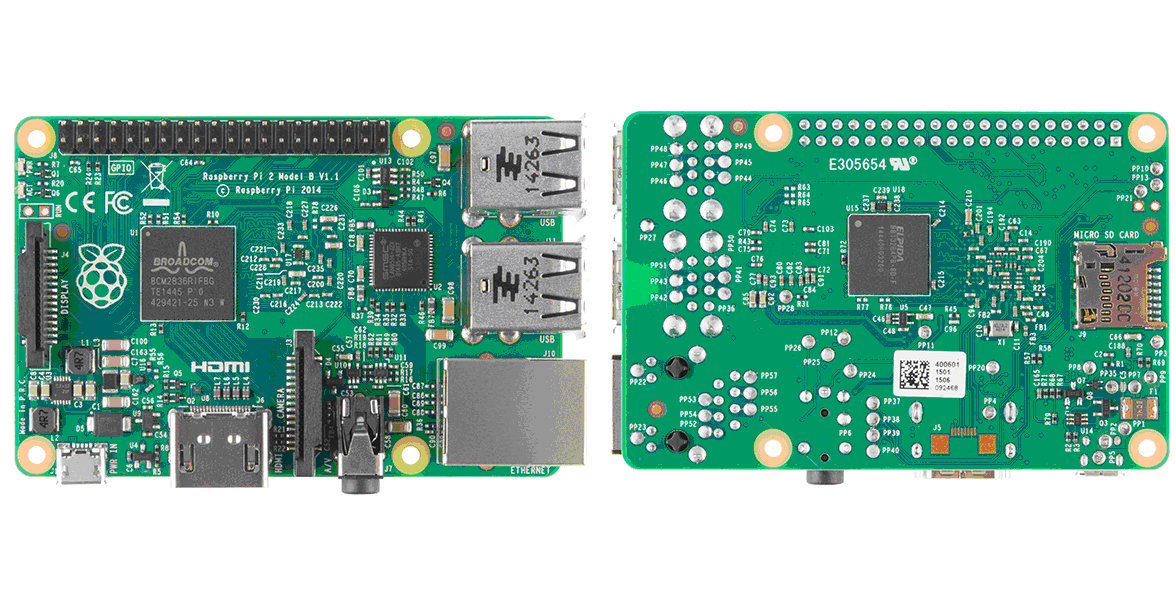
\includegraphics[width=1\textwidth]{figuras/raspberry_pi.png}
\caption{\label{fig:raspberry pi} Raspberry pi 2 modelo B}
\end{figure}

\begin{itemize}
\item{A 900MHz quad-core ARM Cortex-A7 CPU}
\item{1GB RAM}
\item{40 pinos GPIO}
\item{saída Full HDMI}
\item{porta Ethernet}
\item{entrada para cartão Micro SD}
\item{4 entradas USB}
\end{itemize}
%
\subsubsection{Arduino UNO}

Arduino \cite{arduino_site} é uma placa programável open-source. No projeto em questão esse componente receberá os dados do sensor, fará um tratamento e terá o envio programado desses para o coordenador. Pelo Arduino ser programável e possuir uma interface muito amigável, simplifica essa ponte entre a coleta de dados e a transmissão. E sua alta disponibilidade no mercado , assim como o raspberry, facilita sua obtenção. O modelo usado é o UNO (figura \ref{fig:arduino uno})

\begin{figure}[H]
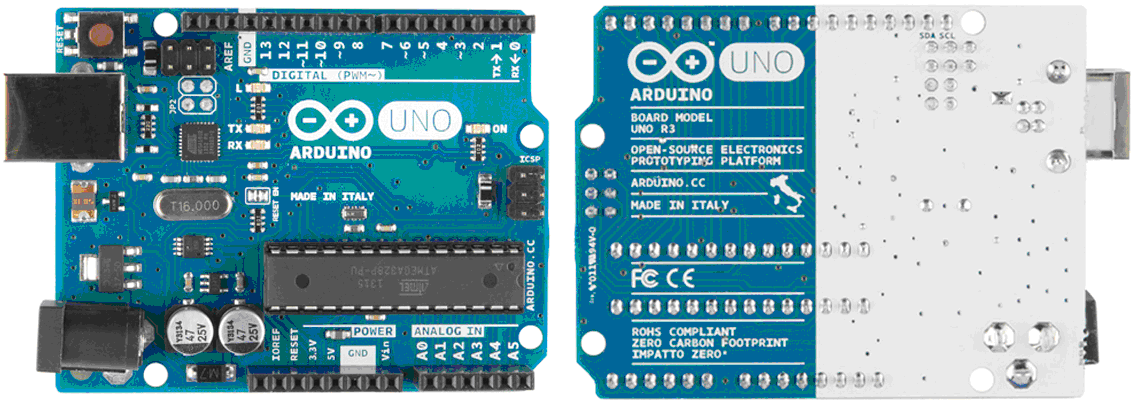
\includegraphics[width=1\textwidth]{figuras/arduino_uno.png}
\caption{\label{fig:arduino uno} Arduino UNO R3}
\end{figure}

\begin{itemize}
\item{microcontrolador ATmega328}
\item{tensão de entrada - 7-12V}
\item{14 Pinos Digital I/O (6 PWM de saída)}
\item{6 Inputs Analógicos}
\item{32k de memória Flash}
\item{16Mhz de Relógio}
\end{itemize}
%
\subsubsection{XBee}

É um módulo que permite uma comunicação simples e confiável entre microcontroladores, computadores, sistemas através de uma porta serial com um consumo menor de energia. Pode ser utilizado em redes ponto-a-ponto e multi-ponto. Foram escolhidos módulos da série 2 (figura \ref{fig:xbee}) por serem configuráveis através de um software da mesma empresa \cite{xctu_software}.

\begin{figure}[H]
\begin{center}
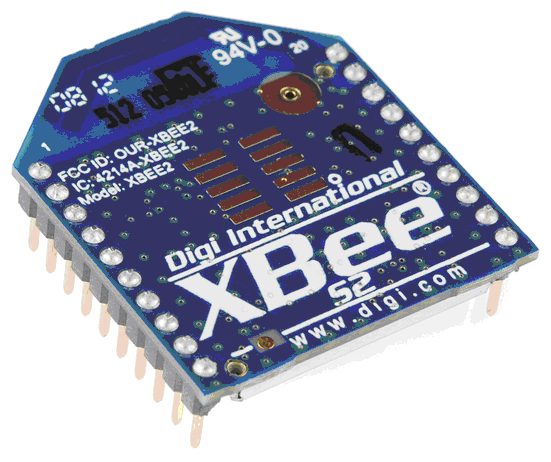
\includegraphics[width=5cm,height=5cm,keepaspectratio]{figuras/xbee_serie2.png}
\caption{\label{fig:xbee} XBee Serie 2}
\end{center}
\end{figure}

Algumas outras especificações são:

\begin{itemize}
\item{entradas de 3.3V @ 40mA}
\item{transmissão de dados máxima de 250kbps}
\item{potência de saída: 2mW (+3dBm)}
\item{alcance máximo de 120m}
\item{08 pinos digitais entrada/saída}
\item{encriptação 128-bit}
\item{configuração local ou remota}
\item{conector de antena RPSMA}
\end{itemize}
%
\subsubsection{XBee Explorer Dongle}

É um módulo com porta USB que faz a conexão do módulo XBee a um computador (figura \ref{fig:xbee explorer dongle}). Isso é necessário para ter acesso aos pinos de comunicação serial e de programação. Ele possui um conversor serial, que traduz os dados entre o computador e o XBee. Possui um botão de reset e um regulador de tensão para suprir a tensão necessária para XBee. Além disso possui 4 leds para debug: RX, TX, RSSI e indicador de energia. No projeto, este módulo é utilizado para fazer as configurações iniciais de todos os XBees e para conectar o XBee coordenador ao Raspberry Pi. Apesar de não ser um dispositivo essencial, este facilita muito nas tarefas citadas,  principalmente por lidar com a alimentação de 3,3V do XBee. Sendo um projeto aberto de hardware, seu desenho esquemático é acessível para uso público \cite{xbee_explorer_dongle_schematic}. 

\begin{figure}[H]
\begin{center}
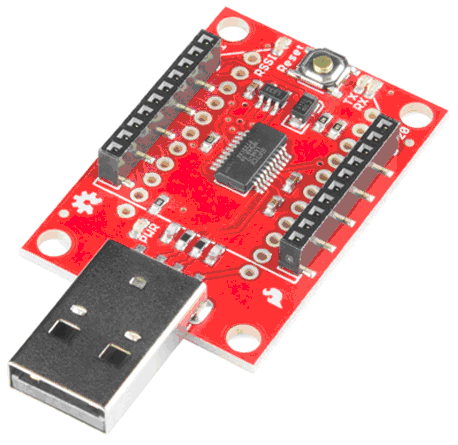
\includegraphics[width=5cm,height=5cm,keepaspectratio]{figuras/xbee_explorer_dongle.png}
\caption{\label{fig:xbee explorer dongle} XBee Explorer Dongle}
\end{center}
\end{figure}

\subsubsection{XBee Shield}

É um módulo que faz a conexão entre um módulo XBee e um Arduino (figura \ref{fig:xbee shield}). Ele possui opções para escolher se a conexão vai ser nos pinos UART ou qualquer outros pinos digitais do Arduino. A alimentação de 5V vinda do Arduino é regulada para 3.3V VDC antes de chegar no módulo XBee. O XBee Shield inclui LEDs para indicar a utilização dos pinos DIN, DOUT, RSSI e DIO5 do XBee. É usado um módulo XBee Shield para cada par XBee + Arduino. Assim como o XBee Explorer Dongle, seu esquemático também é acessível para uso público \cite{xbee_shield_schematic}. 

\begin{figure}[H]
\begin{center}
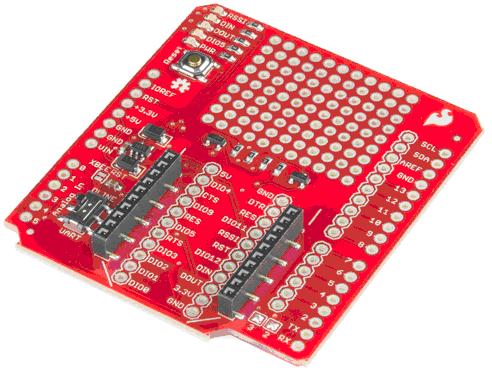
\includegraphics[width=5cm,height=5cm,keepaspectratio]{figuras/xbee_shield.png}
\caption{\label{fig:xbee shield} XBee shield do arduino UNO}
\end{center}
\end{figure}

\subsubsection{Arduino Stackable Header Kit - R3}

São conectores usados para encaixar o módulo XBee Shield no Arduino Uno R3 (figura \ref{fig:xbee shield headers}). Estão inclusos 4 headers, 2 x 8 pinos, 1 x 10 pinos e 1 x 6 pinos, suficientes para 1 módulo XBee Shield. Como há 2 sensores no projeto, serão usados 2 kits, com um adicional de reserva.

\begin{figure}[H]
\begin{center}
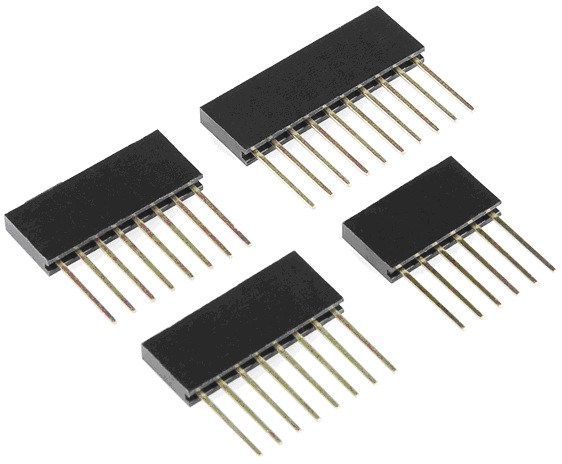
\includegraphics[width=5cm,height=5cm,keepaspectratio]{figuras/headers.png}
\caption{\label{fig:xbee shield headers} Headers usados no XBee shield}
\end{center}
\end{figure}